(\textit{Exercise 6.3 S\&B})
Consider TD(0) run on the random walk example.

(a) (\textit{Exercise 6.3 S\&B}) From the results shown in the left graph, it
appears that the first episode results in a change in only $V(A)$.
What does this tell you about what happened on the first episode?
Why was only the estimate for this one state changed?
By exactly how much was it changed?

%% \textbf{Answer:}
%% The initial estimate $V(A) = 0.5$. Since, the estimate decreases, the episode must have ended in the left terminal state. Let us denote the left terminal state by $L$. Then the last transition of the episode is: $(S=A, R=0, S'=L)$. The update corresponding to this transition is:
%% \begin{IEEEeqnarray*}{lCl}
%%   V(A) &=& V(A) + 0.1 [0 + V(L) - V(A)] \\
%%   &=& 0.5 + 0.1 [0 + 0 - 0.5] \\
%%   &=& 0.45.
%% \end{IEEEeqnarray*}

%% For all other transitions $(S, R=0, S')$ with $S' \notin \{L, R\}$ with $R$ denoting the right terminal state, the updates would be: $V(S) = V(S) + 0.1 [0 + V(S') - V(S)] = V(S)$, since at the beginning of the episode $V(S) = V(S') = 0.5$.


(b) (\textit{Exercise 6.4 S\&B})
The specific results shown in the right graph of the random walk example are dependent on the value of the step-size parameter, $\alpha$. Do you think the conclusions about which algorithm is better would be affected if a wider range of $\alpha$ values were used? Is there a different, fixed value of $\alpha$ at which either algorithm would have performed significantly better than shown? Why or why not?

% MARTHAC: This is too much. Instead, I explain this outloud when discussing 6.4 as an extra bit of info
%(c) \textbf{(Challenge Question, Optional)} (\textit{Exercise 6.5 S\&B}) In the right graph of the random walk example, the RMS error of the TD method seems to go down and then up again, particularly at high $\alpha$s. What could have caused this? Do you think this always occurs, or might it be a function of how the approximate value function was initialized?
\begin{figure}[h!]
\centering

\includegraphics[scale=0.9]{figures/c2m2_rw.pdf}
\end{figure}
\begin{figure}[h!]
\centering
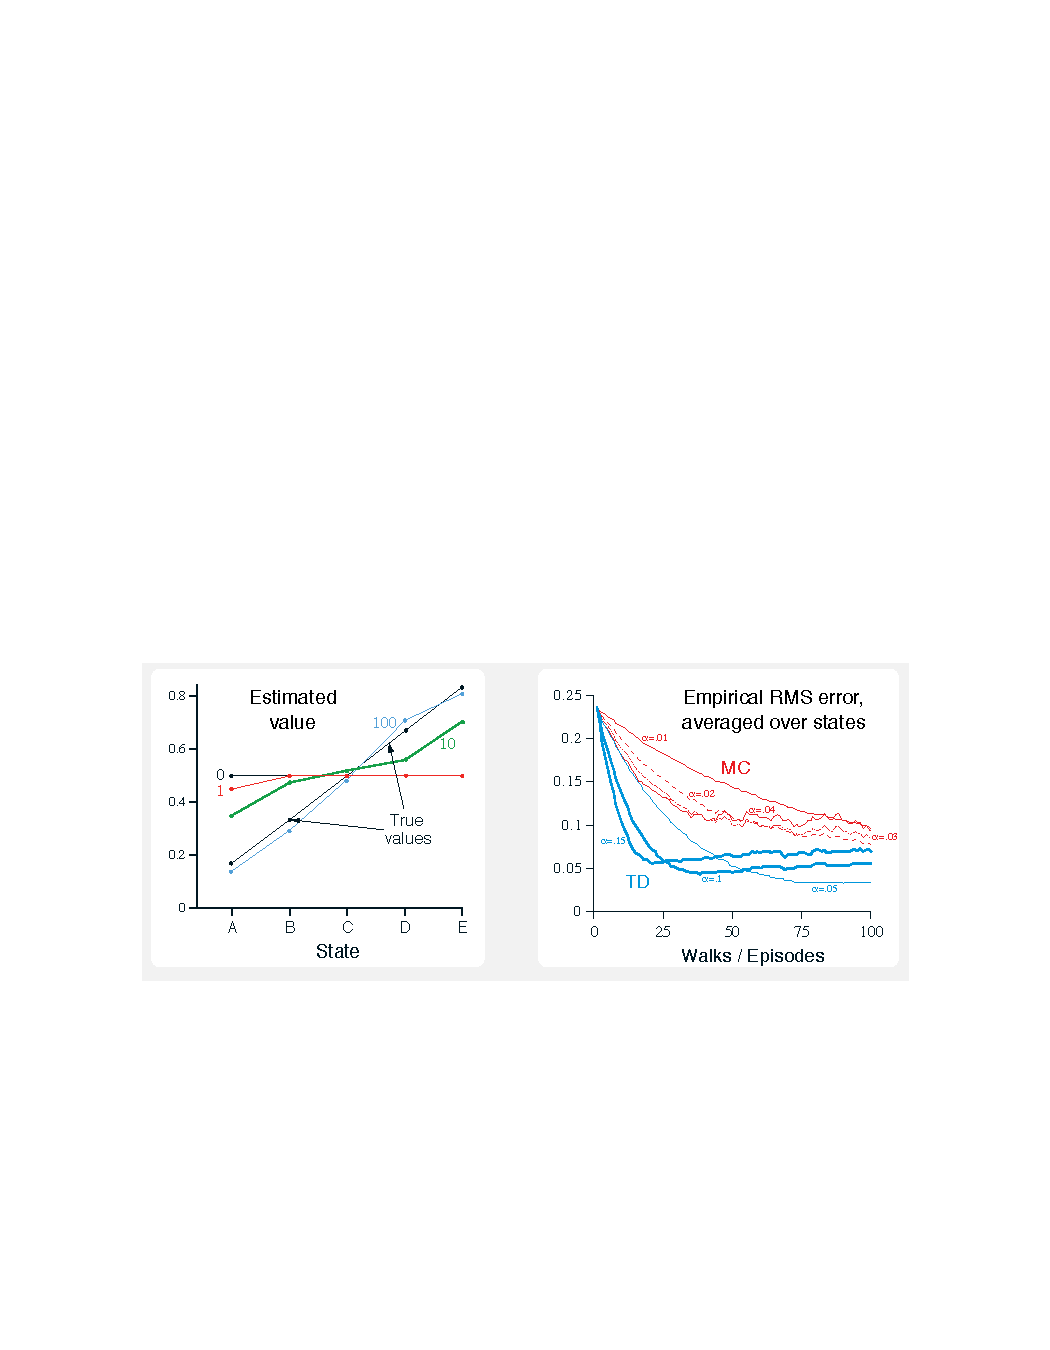
\includegraphics[scale=0.9]{figures/figure_6dot2.pdf}
\end{figure}

%% \textbf{Answer:}
%% Most likely the conclusion that TD is better than Monte Carlo on this method won't change with a wider range of stepsizes. For the MC curve, we can see that the final performance of MC method is best at an intermediate value of $\alpha=0.03$. This is characteristic of performance against parameters (parameter studies) --- an intermediate value of parameters performs better than extreme values. As a result, trying higher and smaller values of $\alpha$ won't likely bring a big difference in the final performance of the MC method. And since the best performance of MC for $\alpha=0.03$ is still worse than the worst TD, the conclusions should remain the same that TD is superior to MC in this setting. Similarly, for TD, tuning the stepsize wouldn't create a big difference in terms of performance. \textcolor{red}{For TD this answer is vague. Maybe add a discussion about TD bounds}.
